\documentclass[11pt]{article}
% Shared preamble of the RMC kernel write-ups (% Shared preamble of the RMC kernel write-ups (% Shared preamble of the RMC kernel write-ups (\input{preamble} after \documentclass).
\usepackage[margin=1in]{geometry}
\usepackage{amsmath,amssymb,bm}
\usepackage{graphicx}
\usepackage{booktabs}
\usepackage{hyperref}

\newcommand{\dd}{\,\mathrm{d}}
\newcommand{\Ein}{E}
\newcommand{\Eout}{E'}
\newcommand{\Ecm}{E_{c}}
\newcommand{\mucm}{\mu_{c}}
\newcommand{\mulab}{\mu_0}

% Common closing section: how the verification figures are produced
\newcommand{\verificationmethod}{%
Each figure is produced by \texttt{verification/verify\_laws.py}. For an incident
energy $\Ein$ along $+z$, $10^6$ collisions are sampled with MC/DC's own reaction
sampler (\texttt{sample\_elastic\_scattering}, \texttt{sample\_inelastic\_scattering}
or \texttt{sample\_fission}), and every emitted neutron is histogrammed in
$48 \times 24$ bins of $(\Eout, \mulab)$, with $\mulab$ the lab cosine to $+z$. The
inverted kernel used by RMC is integrated over the same bins (Gauss--Legendre panels;
two-body lines are split where $\mulab^*(\Eout)$ crosses a cosine edge), multiplied by
the number of collisions, and compared with a $\chi^2$ test over bins with at least 5
expected counts (the rest pooled into one bin). The tables list $\chi^2/\mathrm{dof}$,
its $p$-value, the emitted neutrons per collision (sampled vs.\ the integral of the
inverted kernel), and the largest relative change of a bin integral when the
quadrature panels are doubled. Left panels: outgoing-energy marginal; middle:
lab-cosine marginal; right: per-bin $z = (\text{sampled} - \text{inverted}) /
\sqrt{\text{inverted}}$.}
 after \documentclass).
\usepackage[margin=1in]{geometry}
\usepackage{amsmath,amssymb,bm}
\usepackage{graphicx}
\usepackage{booktabs}
\usepackage{hyperref}

\newcommand{\dd}{\,\mathrm{d}}
\newcommand{\Ein}{E}
\newcommand{\Eout}{E'}
\newcommand{\Ecm}{E_{c}}
\newcommand{\mucm}{\mu_{c}}
\newcommand{\mulab}{\mu_0}

% Common closing section: how the verification figures are produced
\newcommand{\verificationmethod}{%
Each figure is produced by \texttt{verification/verify\_laws.py}. For an incident
energy $\Ein$ along $+z$, $10^6$ collisions are sampled with MC/DC's own reaction
sampler (\texttt{sample\_elastic\_scattering}, \texttt{sample\_inelastic\_scattering}
or \texttt{sample\_fission}), and every emitted neutron is histogrammed in
$48 \times 24$ bins of $(\Eout, \mulab)$, with $\mulab$ the lab cosine to $+z$. The
inverted kernel used by RMC is integrated over the same bins (Gauss--Legendre panels;
two-body lines are split where $\mulab^*(\Eout)$ crosses a cosine edge), multiplied by
the number of collisions, and compared with a $\chi^2$ test over bins with at least 5
expected counts (the rest pooled into one bin). The tables list $\chi^2/\mathrm{dof}$,
its $p$-value, the emitted neutrons per collision (sampled vs.\ the integral of the
inverted kernel), and the largest relative change of a bin integral when the
quadrature panels are doubled. Left panels: outgoing-energy marginal; middle:
lab-cosine marginal; right: per-bin $z = (\text{sampled} - \text{inverted}) /
\sqrt{\text{inverted}}$.}
 after \documentclass).
\usepackage[margin=1in]{geometry}
\usepackage{amsmath,amssymb,bm}
\usepackage{graphicx}
\usepackage{booktabs}
\usepackage{hyperref}

\newcommand{\dd}{\,\mathrm{d}}
\newcommand{\Ein}{E}
\newcommand{\Eout}{E'}
\newcommand{\Ecm}{E_{c}}
\newcommand{\mucm}{\mu_{c}}
\newcommand{\mulab}{\mu_0}

% Common closing section: how the verification figures are produced
\newcommand{\verificationmethod}{%
Each figure is produced by \texttt{verification/verify\_laws.py}. For an incident
energy $\Ein$ along $+z$, $10^6$ collisions are sampled with MC/DC's own reaction
sampler (\texttt{sample\_elastic\_scattering}, \texttt{sample\_inelastic\_scattering}
or \texttt{sample\_fission}), and every emitted neutron is histogrammed in
$48 \times 24$ bins of $(\Eout, \mulab)$, with $\mulab$ the lab cosine to $+z$. The
inverted kernel used by RMC is integrated over the same bins (Gauss--Legendre panels;
two-body lines are split where $\mulab^*(\Eout)$ crosses a cosine edge), multiplied by
the number of collisions, and compared with a $\chi^2$ test over bins with at least 5
expected counts (the rest pooled into one bin). The tables list $\chi^2/\mathrm{dof}$,
its $p$-value, the emitted neutrons per collision (sampled vs.\ the integral of the
inverted kernel), and the largest relative change of a bin integral when the
quadrature panels are doubled. Left panels: outgoing-energy marginal; middle:
lab-cosine marginal; right: per-bin $z = (\text{sampled} - \text{inverted}) /
\sqrt{\text{inverted}}$.}


\title{Inverted kernel: simple Maxwellian fission spectrum (ENDF Law 7)}
\date{}

\begin{document}
\maketitle

\noindent Code: \texttt{evaluate\_maxwellian}, \texttt{maxwellian\_normalization} in
\texttt{mcdc/rmc/evaluate.py}.

\section{What MC/DC samples}

\texttt{sample\_maxwellian}: with $\theta(\Ein)$, $U$, $L = \Ein - U$ as for the
evaporation spectrum,
\begin{equation}
  x = -\theta\left[\ln\xi_1 + \ln\xi_2\cos^2\!\left(\tfrac{\pi}{2}\xi_3\right)\right],
  \qquad\text{accepted if } 0 \le x \le L .
\end{equation}

\section{Density of the sampled value}

$-\ln\xi_1$ is $\mathrm{Gamma}(1)$. For $\xi_3$ uniform, $B = \cos^2(\pi\xi_3/2)$ has
the arcsine density $1/(\pi\sqrt{b(1-b)})$, i.e.\ $B \sim \mathrm{Beta}(\tfrac12,
\tfrac12)$, and the beta--gamma algebra
$\mathrm{Gamma}(a+b)\cdot\mathrm{Beta}(a, b) \sim \mathrm{Gamma}(a)$ (independent
factors) with $a = b = \tfrac12$ gives $-\ln\xi_2\,B \sim \mathrm{Gamma}(\tfrac12)$.
The sum of independent $\mathrm{Gamma}(1)$ and $\mathrm{Gamma}(\tfrac12)$ is
$\mathrm{Gamma}(\tfrac32)$, so $x/\theta \sim \mathrm{Gamma}(\tfrac32)$ before
rejection, with density $\propto\sqrt{x}\,e^{-x/\theta}$. Restricting to $[0, L]$,
\begin{equation}
  p(x \mid \Ein) = \frac{\sqrt{x}\,e^{-x/\theta}}{\theta^{3/2} I(w)},\qquad
  I(w) = \int_0^w\sqrt{s}\,e^{-s}\dd s
  = \frac{\sqrt\pi}{2}\operatorname{erf}(\sqrt w) - \sqrt w\,e^{-w},
  \qquad w = \frac{\Ein - U}{\theta},
\end{equation}
with $I(w) = w^{3/2}\left(\tfrac23 - \tfrac25 w + \tfrac17 w^2\right)$ for
$w < 10^{-3}$. Support $[0, \Ein - U]$; the density is smooth inside it (its
$\sqrt{x}$ endpoint behaviour limits Gauss--Legendre accuracy only in a bin touching
$\Eout = 0$). Reaction kernel as for evaporation: $Y p\,p_\mu$ in the reaction's frame.

\paragraph{Data.} No nuclide in the 293.6\,K library uses Law 7, so the verification
uses C-12 MT-91 with its evaporation spectrum relabelled as Maxwellian (same
$\theta(\Ein)$ and $U$). The generator wrote the Maxwellian interpolation laws under
\texttt{temperature\_interpolation} while the loader read
\texttt{temperature\_interpolations}; \texttt{fix/evaporation-maxwellian-loading}
unifies the name (the loader accepts both).

\section{Verification}
\verificationmethod

\begin{center}
\begin{tabular}{rrrrrrr}
\toprule
$E$ [eV] & samples & bins & $\chi^2/\mathrm{dof}$ & $p$ & yield (sampled / inverted) & quad. err. \\
\midrule
1.2e+07 & 1e+06 & 769 & 768.5/769 & 0.498 & 1.00000 / 1.00000 & 2.1e-05 \\
1.8e+07 & 1e+06 & 745 & 730.0/745 & 0.646 & 1.00000 / 1.00000 & 2.2e-05 \\
\bottomrule
\end{tabular}

\end{center}

\begin{figure}[h]
  \centering
  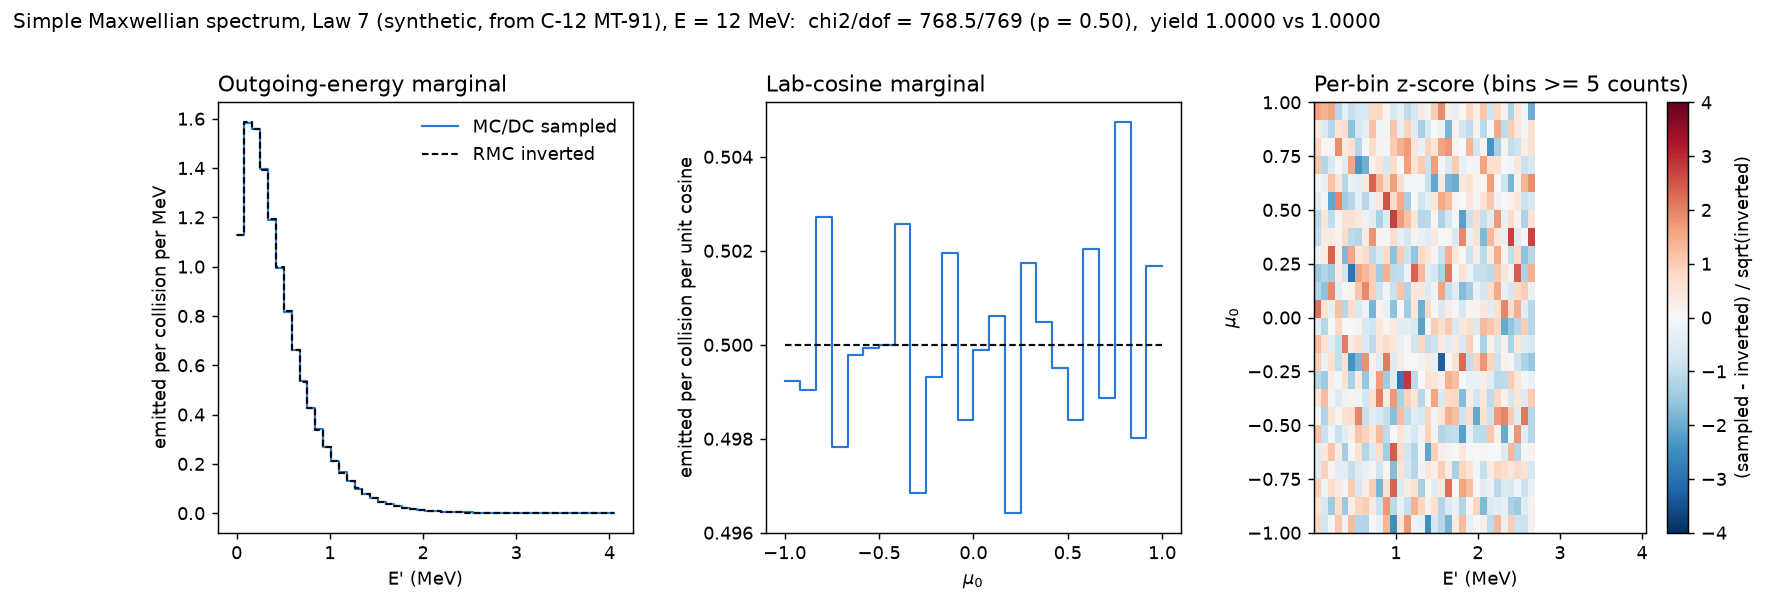
\includegraphics[width=\textwidth]{figures/maxwellian/maxwellian_E1p2e07.png}
  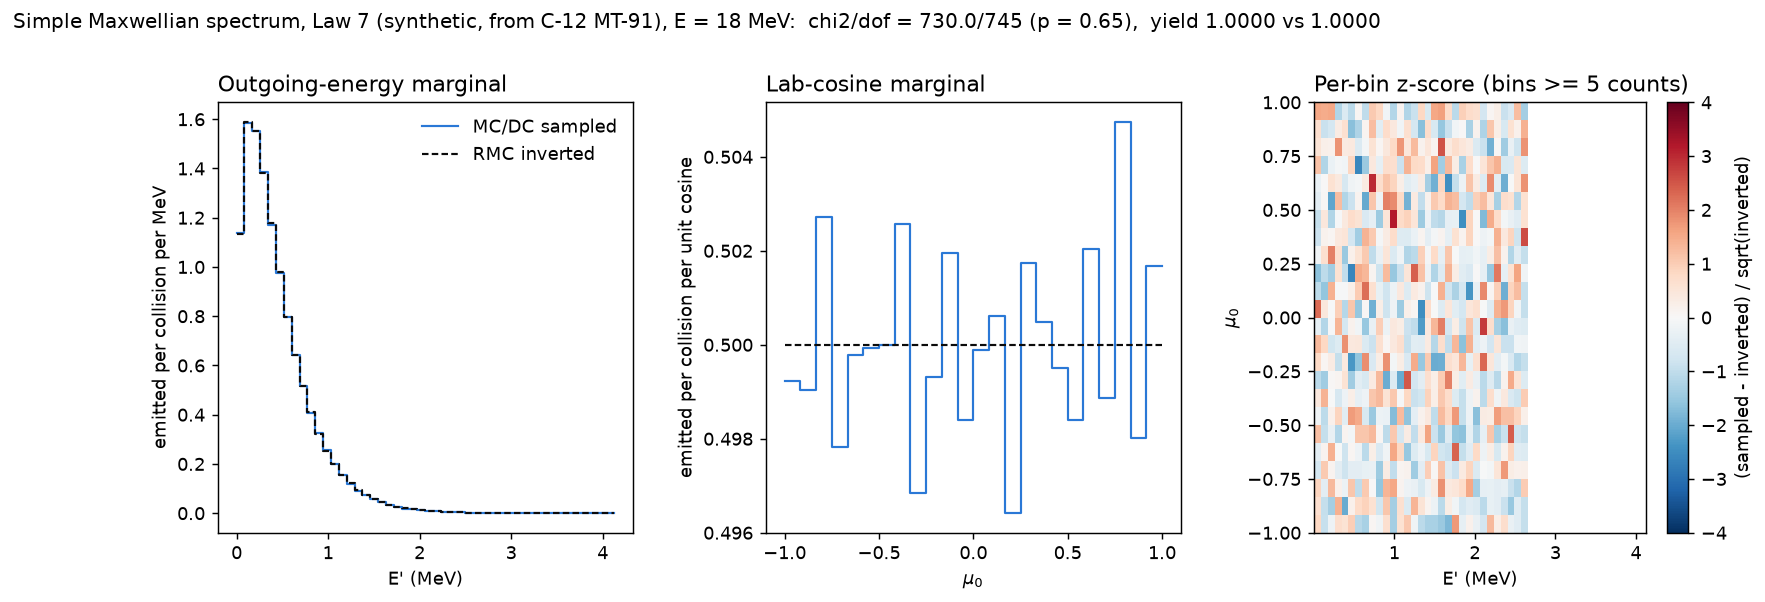
\includegraphics[width=\textwidth]{figures/maxwellian/maxwellian_E1p8e07.png}
  \caption{Maxwellian spectrum ($\theta = 0.3$\,MeV, $U = 7.89$\,MeV, lab frame,
  isotropic) at 12 and 18\,MeV.}
\end{figure}

\end{document}
